\section*{Introduction}

Compton scattering represents the main  type of $\gamma$-matter interaction with $\gamma$ energy of the MeV order.   
The aim of this experiment is to present the study of Compton Scattering performed with the experimental Set Up described in the following section.
This report will analyze these steps:
\begin{itemize}
	\item Energy calibration of the three inorganic scintillators.
	\item Verification of the relationship between energy and angle of the diffused photon.
	\item Measure of the differential cross section of Compton Scattering.
\end{itemize}

\section*{Experimental Set Up}

To study the Compton scattering three inorganic NaI(Tl) scintillators with 7.5~cm diameter and height were used.  upled with a Photonics Photomultiplier XP2020~(see Fig.~\ref{fig:Set_up}). The anode outputs of the PMT were sent to a Quad Linear Gate FAN-IN/OUT mod. Philips 744 in order to split them. One output then was sent directly to a CAEN digitizer mod. DT5751, an ADC with a sampling rate of 1 Gs/s and a resolution of 10 bit, while the other one was sent to a Quad CFD mod. 935. The timing signals obtained from the CFD unit were processed by a CAEN Quad Logic Unit mod. N455 to produce a coincidence signal between the two detectors, used as trigger input for the digitizer. They were also to sent to an Ortec TAC unit to measure their time difference. The output of the TAC module was also digitized.

\begin{figure}[h!]
	\centering
	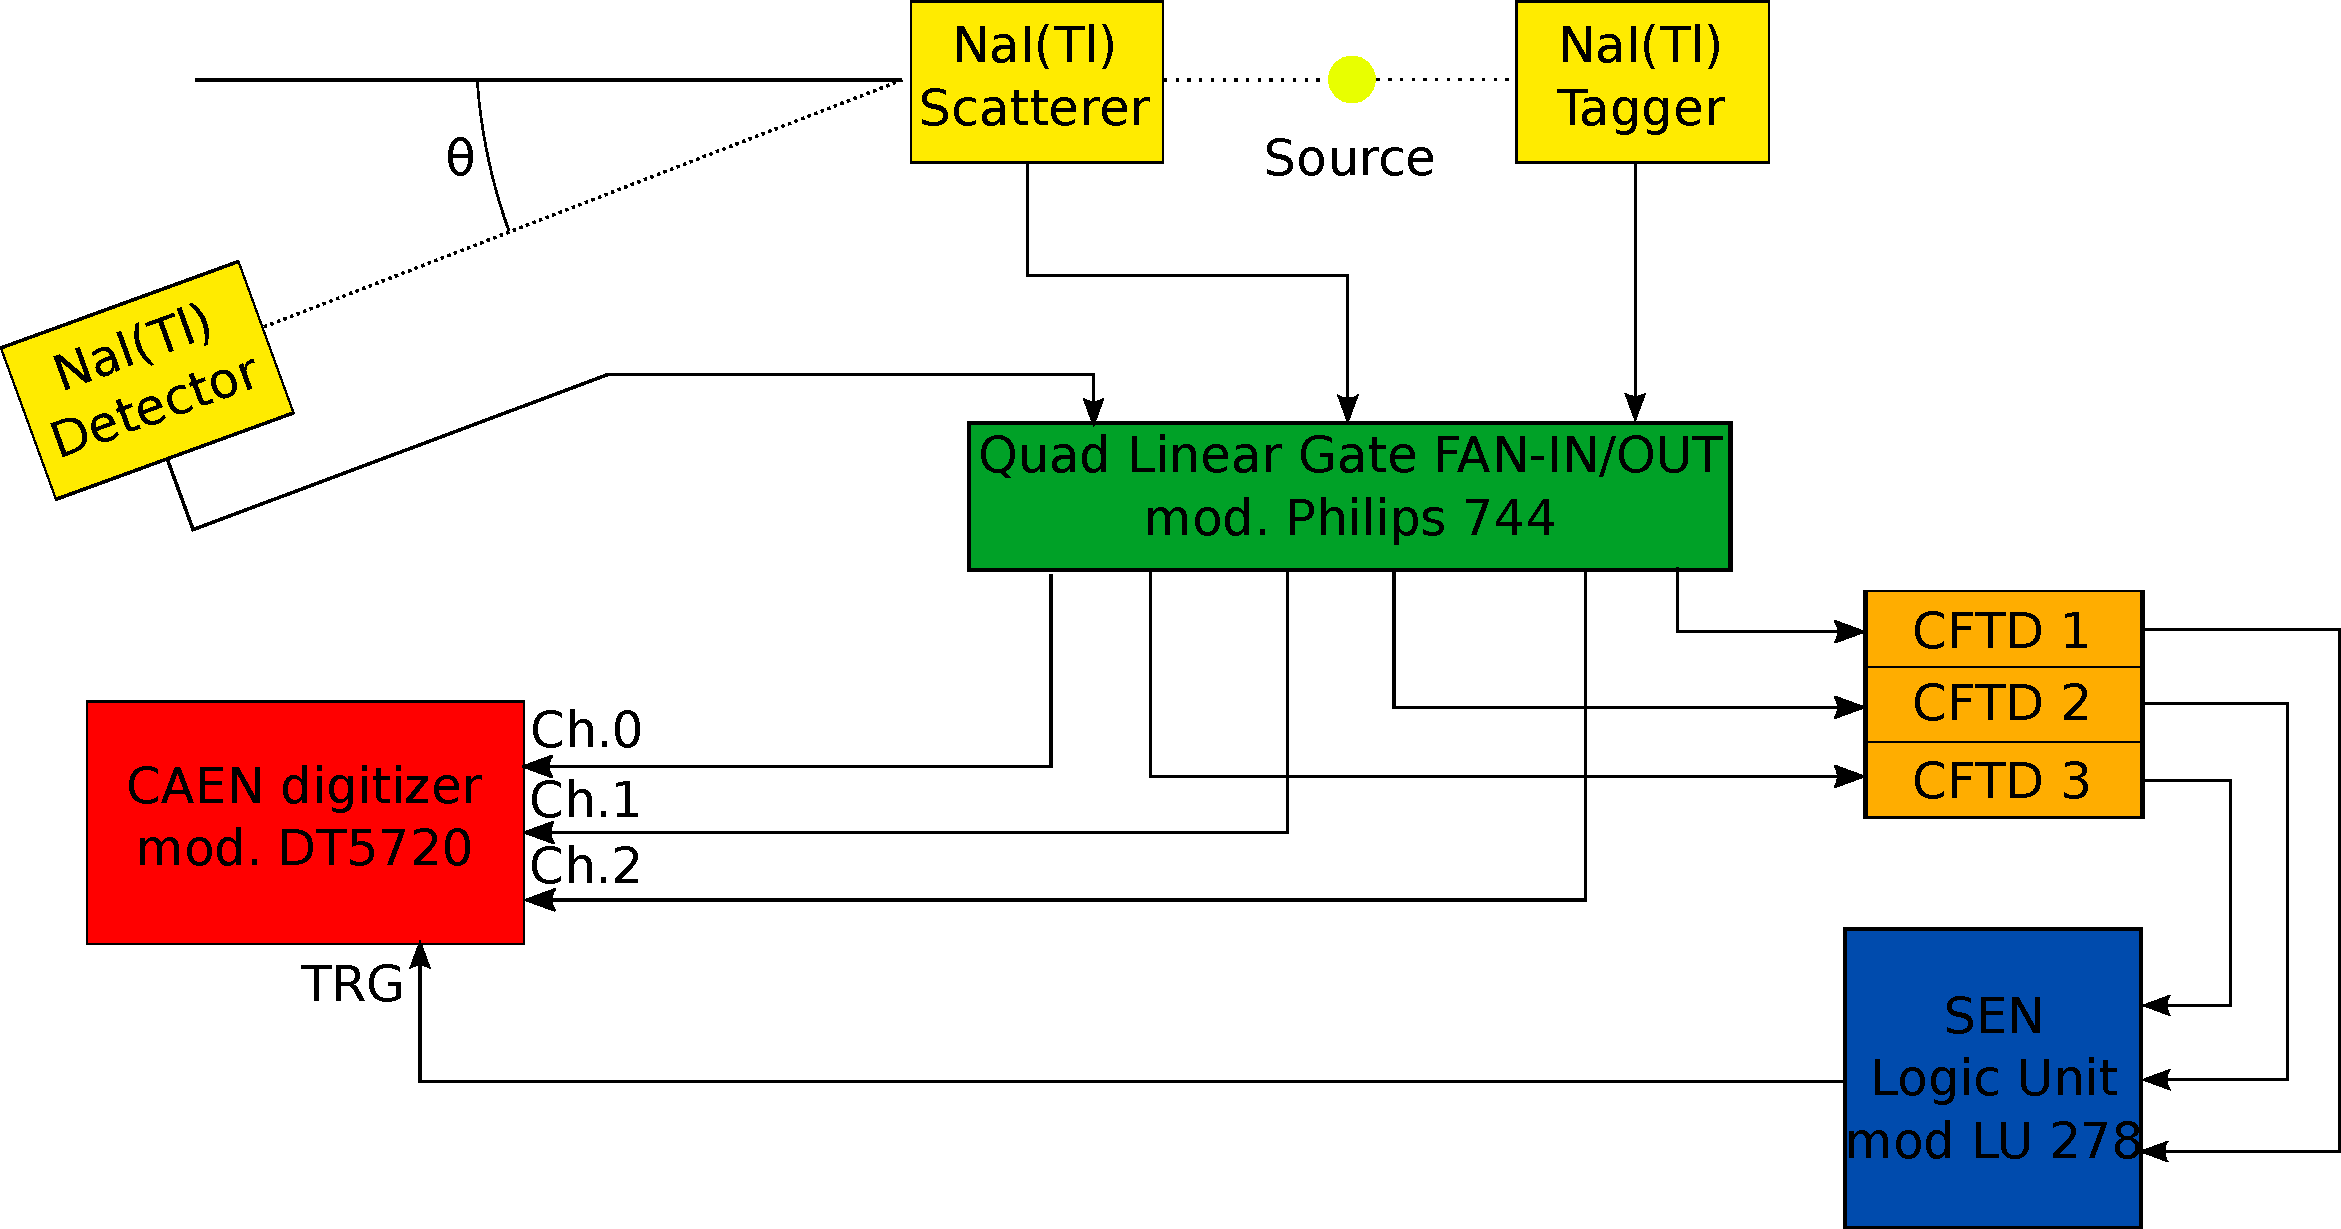
\includegraphics[width=\textwidth]{immagini/SetUp.pdf}
	\caption{Experimental configuration adopted for the Compton Scattering experiment.}
	\label{fig:Set_up}
\end{figure}